\section{Architecture}
\label{sec:corearchitecture}

The first versions of CORE used FreeBSD's jails, one of the first container systems in UNIX-like operating systems, to create virtual nodes with a small computational resources \cite{comparisonofcore,freebsdjails}.
Currently, CORE is a Linux-only solution and uses the Linux containers (LXC) set of technologies, namely network namespaces, as the underlying OS support for node virtualiztaion and emulation~\cite{coreghdocs}.

A set of low-level primitives allows to create separated networking stacks (the aforementioned namespaces, \texttt{netns}) in the same host's kernel, also sharing the filesystem, but binding separate instances of specific processes---like routing daemons or any other software that communicates with the network---to those namespaces.

The control of the nodes' creation and spawning of processes bound to those nodes, as well as passing shell commands to inside the containers, and also creating virtual links using inter-container bridges, is done by the \emph{core-daemon} program.
This ``part'' of the CORE infrastructure is its backend.

The other main piece of CORE is its \gls{gui}, \emph{core-gui}, which communicates with the core-daemon through a gRPC API~\cite{grpc}.

% Figure fig:core-architecture
\begin{figure}
  \centering
  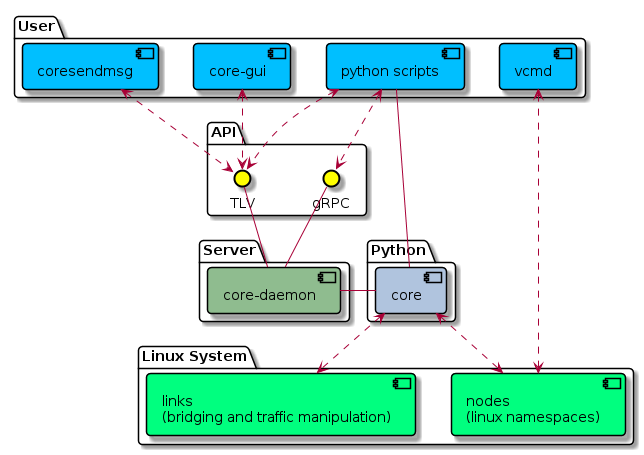
\includegraphics[width=0.8\textwidth]{core-architecture}
  \caption{CORE's architecture diagram taken from the documentation}
  \label{fig:core-architecture}
\end{figure}


Figure \ref{fig:core-architecture}, available from~\cite{coreghdocs}, gives the full picture of all the components of this emulator framework.

% end of section
